\ifx\isEmbedded\undefined

\documentclass[12pt]{report}
	
% FONT RELATED
%\usepackage{times} %Move to times font
\usepackage[labelfont=bf,textfont=it]{caption}
\usepackage[utf8]{inputenc}

% LINKS, PAGE OF CONTENT, REF AND CROSS-REF, HEADERS/FOOTERS
\usepackage[hidelinks]{hyperref}
\usepackage{fancyhdr}
\usepackage{acronym}

% FIGURES, GRAPHICS, TABLES
\usepackage{graphicx}
\usepackage{parskip}
%\usepackage{subfigure}
\usepackage{subfig}
\usepackage{wrapfig}
\usepackage{subfloat}

% COLOURS, TEXT AND FORMATTING
\usepackage{array}
\usepackage{color}
\usepackage{setspace}
\usepackage{longtable}
\usepackage{multirow}

% ADVANCED MATHS, PSEUDO-CODE
\usepackage{amsmath}
\usepackage{alltt}
\usepackage{amsfonts}

% BIBLIOGRAPHY
\usepackage[authoryear]{natbib}
\bibpunct{(}{)}{;}{a}{,}{,}

% USE IN DISSER:

\setlength\oddsidemargin{0.85cm}
\setlength\evensidemargin{0.85cm}

\setlength\textheight{21.0cm}
\setlength\textwidth{15.0cm}

% indent at each new paragrapg
\setlength\parindent{0.5cm}

\setlength\topmargin{-0.2in}
\renewcommand{\baselinestretch}{1.3}

%REPORT

%\setlength\oddsidemargin{1cm}
%\setlength\evensidemargin{0.3in}
%%\setlength\headsep{2.5in}
%
%\setlength\textheight{9.0in}
%\setlength\textwidth{5.5in}
%
%% indent at each new paragrapg
%\setlength\parindent{0.5cm}
%
%%\setlength{\parskip}{10.5ex}
%
%\setlength\topmargin{-0.2in}

%\newcommand{\HRule}{\rule{\linewidth}{0.5mm}}
\newcommand{\HRule}{\rule{\linewidth}{0.0mm}}

% Color definitions (RGB model)
\definecolor{ms-comment}{rgb}{0.1, 0.4, 0.1}
\definecolor{ms-question}{rgb}{0.4, 0.0, 0.0}
\definecolor{ms-new}{rgb}{0.2, 0.4, 0.8}


\graphicspath{{../img/}}
\begin{document}
\fi

\chapter{Agent-Based Model}
\label{chap:agent-based model}

After an introductory chapter and a background overview, this is where this document starts dealing with the particular approach studied in this thesis. The solution will be presented following a bottom-up explanation line, since the author believes that it will be clearer for the reader. Thus, in this chapter the abstract model for an individual which belongs to a crowd, and which lives in the virtual world, is explained into details. This individual, which from now on will be referred as \emph{agent}, is the element that will encapsulate the intelligence of the system. Therefore, this approach is based on individual intelligent agents rather than any global mechanism, from whose interactions a group behaviour will arise. As stated before, the crowd behaviour will have as much quality as the agent behaviours have.

Next Chapter will take a wider vision presenting the concept of crowd and the world which holds the complete simulation.

Since the old Greece, some philosophers argued about a spiritual division between soul and body, other scientists consider the ability of thinking something that escapes the bounds of the physical body. Without going such further, this thesis presents an abstract agent model divided in two parts: a body and a brain.

\section{Agent Body}

This part is the one which is materially in the world, and there is no intelligence in here. It is completely physically based and most of its attributes are immutable during a simulation. The body represents how big an agent is, or how fast it is, etc. This way, an agent might be big and slow or small and fast. These attributes might even limit the capacity of decision of the thinking partition of the agent. Let us imagine a situation where a prey's brain desperately keeps requesting for increasing the velocity to escape from a predator, but the body cannot perform a higher speed. Next, the list of the physical properties which define the body of an agent are presented:

\subsection{Physical Properties}

\begin{itemize}

\item{{\bf Mass.} The mass of an agent determines how much acceleration a force produces on it.
Taking the assumption that agents have comparable densities, it is also employed to visualize their size}

\item{{\bf Strength.} This will influence in the \emph{prime mover force}, which is the force an agent applies on itself to move in the space. Therefore, having agents with the same mass, the strong ones will have the ability of opposing to external forces easily or to produce more self-acceleration, changing their velocity faster. The strength might vary if, for example, the agent gets tired or receives any sort of damage.}

\item{{\bf Maximum Strength.} This is the amount of strength that an agent has when it is fully recovered.}

\item{{\bf Velocity.} This is the current velocity that an agent possesses and, contrary to the strength, this attribute has both magnitude and direction. This is the rate of change of the agent's location; thus, it is used to obtain the next position. It is calculated with the acceleration that the total force produce on the agent.}

\item{{\bf Maximum Speed.} This is the higher punctual speed that an agent can move in the world with. Do not confuse this with how fast an agent can change of physical state, which is related with forces and mass (acceleration). Consider the next example: a cheetah can change from 0 to 100 km/h in a matter of seconds (high acceleration); on the other hand, a high-speed train, which needs a lot of force (strength with direction) to move such a big mass, has much smaller acceleration, but it can travel at 200 km/h (high maximum speed).}

\item{{\bf Vision Radius.} This property determines which portion of the world the agent is aware of. This is mainly used to calculate the other agents that one agent can perceive, which will conform its neighbourhood. Therefore, an explorer may have a large vision radius, meanwhile a blind agent will have vision radius 0, and will need to receive information about the world by other means, such as somebody whispering at its ear (message passing).}

\end{itemize}

\begin{figure}[!htb]
  \centering
  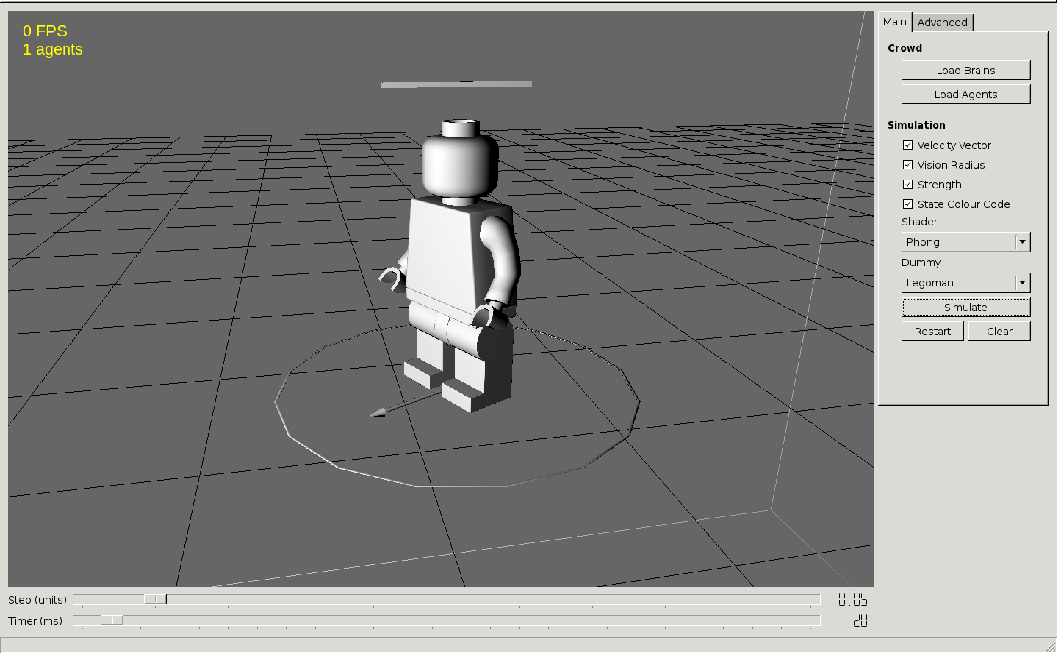
\includegraphics[scale=0.3]{agent.eps}
  \caption{One single agent with its physical properties}
  \label{fig:navigation}
\end{figure}

At this point, a comment regarding to the developing of this method might be pertinent. How an agent's body behaves in the virtual world is uniquely ruled by physical laws. The brain might say ``move up'' and apply a force towards the sky but if this force is smaller than the gravity, then the agent will descend. Hence, the piece of this system relative to the physical simulation or the physical properties of an agent is something static, a fixed and solid structure which works. That is why it is implemented in a compiled language. Nevertheless, somebody's way of thinking or acting, might be so diverse that it needs a flexibility that a compiled language cannot provide.\footnote{Although the design and implementation of the approach are treated in chapter \ref{chap:application_design_implementation}, the author believes that it is convenient to mention some implementations details which are important to understand how much flexibility or scalability this approach offers.}

\section{Agent Brain}
This is where resides the ``intelligence'' of the agent. This piece has the responsability of determining which motion an agent describes, how to interact with the world and how to interact with other agents.

The main mechanism used to model a brain is a FSM, although any other device might be used such as an artificial neural network, which is the closer to reality. This computational box receives a set of information both from the body and from the environment. This includes the physical properties, the current state of the agent, a table of own attributes, a list with its neighbours and their information and a list of the incoming messages. After processing, the brain will communicate to the body what to do by returning certain parameters.

\begin{itemize}

\item{{\bf Prime Mover Force.} This is the brain sends to the body in order to perform a specific displacement. This will be explained into details in the next chapter during the section of forces, but it is basically the force that the muscles should apply on the body to move it in a certain direction and with certain acceleration. The direction is a free choice, but the magnitude should be influenced by the current strength to acquire a realistic motion}

\item{{\bf Heading.} The brain can set the heading of the agent too; this is normally established by the velocity, but there are some kind of motions, such as lateral movements, where the heading does not point in the same direction than the velocity.}

\item{{\bf Strength.} According to this model, it is the brain who decides how much strength the actions of the agent consume or, by the contrary, how fast it recovers. So the new strength is returned.}

\item{{\bf State.} The brain will tell to the body the its new state, which might be the old one, or a new one if some transition was triggered.}

\item{{\bf Messages.} A list with the messages to send to the agent's neighbours. This messages has certain type of information detailed later, and if the receiver knows how to react upon it, its behaviour may be affected}

\end{itemize}

This is where the usability and beauty of the approach arises. The behaviours are script based; therefore, having all the gears of the system spinning properly, any new brain can be added at any time. For the behaviours proposed, it was chosen to use a FSM, as a simple and effective mechanism, but any other more sofisticated method could be used. Different techniques such as movement prediction, statistical study, evolving algorithms, etc. might be employed for developing new agent behaviours and observe the emergent configuration of the crowd.

\subsection{Capacity of Decision}

This is what, under a physical consistency, drives the simulation. The ability that an agent has to take decisions is the main input to produce a simulation. If we have in mind any simple video game in where we control a character to interact with a world, we are taking decisions, tons of them. They might be long term ones (reach a target) or short term ones (this way seems a shortcut). Thus, the idea is automate this task. An infinite amount of things might influence every decision we take in real life: in which state we feel, where we are, how tired we are, which is our physical shape, who is surrounding us, what we know about who is surrounding us, etc. In order to take accurate decisions a large amount of information needs to be taken into account, besides all the different possibilities available; but that could produce extremely complex FSM's or other artifacts very difficult to handle.

\subsection{The Illusion of Intelligence}

Intelligence is a very complex concept. It is thought as a mental capability that involves things such as the ability to reason, plan, solve problems, think abstractly, comprehend complex ideas, learn quickly or learn from experience.

The decisions an agent takes and behaviour it presents during time will tell us if it is intelligent or not. Building a simple behaviour is a matter of minutes, building a very intelligent behaviour might require several times the time this thesis was done in.


\section{Interaction among agents. Message passing}

me

\section{Overview of Possible Behaviours}

some basic ones and the own ones


\ifx\isEmbedded\undefined
% References
\addcontentsline{toc}{chapter}{References}
\bibliographystyle{../ref/harvard}
\bibliography{../ref/master}
\pagebreak
\end{document}
\fi